\documentclass[a4paper]{article}
%\usepackage[singlespacing]{setspace}
\usepackage[onehalfspacing]{setspace}
%\usepackage[doublespacing]{setspace}
\usepackage{geometry} % Required for adjusting page dimensions and margins
\usepackage{amsmath,amsfonts,stmaryrd,amssymb,mathtools,dsfont} % Math packages
\usepackage{tabularx}
\usepackage{colortbl}
\usepackage{listings}
\usepackage{amsmath}
\usepackage{amssymb}
\usepackage{amsthm}
\usepackage{subcaption}
\usepackage{float}
\usepackage[table,xcdraw]{xcolor}
\usepackage{tikz-qtree}
\usepackage{changepage,titlesec,fancyhdr} % For styling Header and Titles
\pagestyle{fancy}

\usepackage{enumerate} % Custom item numbers for enumerations

\usepackage[ruled]{algorithm2e} % Algorithms

\usepackage[framemethod=tikz]{mdframed} % Allows defining custom boxed/framed environments

\usepackage{listings} % File listings, with syntax highlighting
\lstset{
	basicstyle=\ttfamily, % Typeset listings in monospace font
}

\usepackage[ddmmyyyy]{datetime}


\geometry{
	paper=a4paper, % Paper size, change to letterpaper for US letter size
	top=2.5cm, % Top margin
	bottom=3cm, % Bottom margin
	left=2.5cm, % Left margin
	right=2.5cm, % Right margin
	headheight=25pt, % Header height
	footskip=1.5cm, % Space from the bottom margin to the baseline of the footer
	headsep=1cm, % Space from the top margin to the baseline of the header
	%showframe, % Uncomment to show how the type block is set on the page
}
\lhead{ALGO-1\\Sommersemester 2024}
\chead{\bfseries{Übungsblatt 6}\\}
\rhead{7987847\\Jonas Werner}

\begin{document}
\section*{Aufgabe 6.1}
Wir betrachten die folgende Liste von Integern
\begin{center}
    12, 30, 60, 8, 14, 55, 90, 10
\end{center}
\subsection*{a)}
Hat die Liste Heap-Order?

\begin{tikzpicture}[level/.style={sibling distance=60mm/#1, circle, draw}]
\node {12}
  child {
    node {30} 
    child {
      node {8}
      child {
        node {10}
      }
    }
    child {
      node {14}
    }
  }
  child {
    node {60}
    child {
      node {55}
    }
    child {
      node {90}
    }
  };
\end{tikzpicture}

Nein, die Liste hat keine Heap-Order. Die Kinder der Wurzel sind beide größer als die Wurzel, daher kann ab diesem Punkt die Heap-Order nur der eines Min-Heaps entsprechen, jedoch ist sind Prioritäten der Kinder des Knoten $30$ kleiner als die des Knoten selbst. Dadurch kann die Liste keine Heap-Order haben.


\subsection*{b)}
Fügen Sie die Integer der Reihe nach in einen zu Beginn leeren Max-Heap ein. Geben Sie den
Heap nach jeder $repair\_up()$ Operation als Array an.\\

Liste $\rightarrow$ Liste nach $repair\_up()$
\begin{enumerate}
    \item $[] \rightarrow []$
    \item $[12] \rightarrow [12]$
    \item $[12, 30] \rightarrow [30, 12]$
    \item $[30, 12, 60] \rightarrow [60, 12, 30]$
    \item $[60, 12, 30, 8] \rightarrow [60, 12, 30, 8]$
    \item $[60, 12, 30, 8, 14] \rightarrow [60, 14, 30, 8, 12]$
    \item $[60, 14, 30, 8, 12, 55] \rightarrow [60, 14, 55, 8, 12, 30]$
    \item $[60, 14, 55, 8, 12, 30, 90] \rightarrow [90, 14, 60, 8, 12, 30, 55]$
    \item $[90, 14, 60, 8, 12, 30, 55, 10] \rightarrow [90, 14, 60, 10, 12, 30, 55, 8]$
\end{enumerate}

\subsection*{c)}
Führen Sie auf dem Heap aus Aufgabenteil b) $change\_priority(3, 40)$ aus. Welche Operationen sind zur Reparatur auszuführen? Geben Sie den Heap nach der Ausführung von $change\_priority()$ sowie nach jeder weiteren ausgeführten Operation als Array an.\\

[90, 14, 60, 10, 12, 30, 55, 8]\\

$change\_priority(3, 40) \rightarrow$ [90, 14, 40, 10, 12, 30, 55, 8]\\

Um die Heap-Order zu reparieren muss folgender Schritt gemacht werden:\\

$repair\_up(55) \rightarrow$ [90, 14, 55, 10, 12, 30, 40, 8]


\break

\section*{Aufgabe 6.2}
Im Folgenden betrachten wir eine Verallgemeinerung der in der Vorlesung diskutieren binären Heaps. In sogenannten \textit{k-nären} Heaps, wobei $k \geq 3$, gilt weiterhin die Heap-Ordnung. Jedoch ändert sich die Heap-Struktur: In einem \textit{k-nären} Heap der Tiefe $t$ hat jeder Knoten in Tiefe höchstens $t - 2$ genau $k$ Kinder (statt genau zwei Kindern bei binären Heaps). In Tiefe $t - 1$ gibt es einen Knoten $v$ mit höchstens $k$ Kindern. Alle Knoten in Tiefe $t - 1$ links des Knotens $v$ haben genau $k$ Kinder; alle Knoten in Tiefe $t - 1$ rechts von $v$ sind Blätter.

\subsection*{a)}
Zeigen Sie, dass die Tiefe des zugehörigen Baums mit n Knoten $\theta(\log_k n)$ beträgt.
TODO

\subsection*{b)}
Geben sie an,
\subsubsection*{i)}
in welcher Position im Array sich die Kinder von Knoten $i$ für $1 \leq i \leq n$ befinden (sofern sie existieren),\\

Wir benötigen eine Hilfsvariable $s$ welche das $s-te$ Kind des Knoten $i$ meint.\\

$s \in \mathbb{N} | (1, k)$\\

Somit ist die Formel um den Index für das $s-te$ Kind des Knoten $i$ zu bekommen:

$index = i \cdot k - (k-s + 1)$

\subsubsection*{ii)}
in welcher Position im Array sich der Elternknoten von Knoten $j$ für $2 \leq j \leq n$ befindet.\\

Für diese Formel benötigen wir die floor-Notation $\lfloor \cdot \rfloor$ weil je nachdem bei welchem Kind wir sind, ist der Index dieses Kindes näher bei dem des Vaters oder weiter weg. Dabei muss dann abgerundet werden.\\

Die Formel lautet dann:\\

$index = \lfloor \frac{i + (k - 2)}{k}\rfloor$

\subsection*{c)}
Passen Sie die Prozedur $repair\_down()$ so an, dass sie für \textit{k-näre} Heaps funktioniert. Beschreiben Sie
die geänderte Prozedur in Pseudocode und analysieren Sie die Laufzeit Ihres Verfahrens asymptotisch in $k$ und $n$.

\begin{verbatim}
    void heap::repair_down (int wo, k)
    {
        int kind; int p = H[wo];
        while (wo <= n/2 && wo * k - (k - kind + 1) > p)
        {
            kind = 2 * wo;
            if ((kind < n) && (H[kind] < H[kind + 1])) kind ++;
            if (p >= H[kind]) break;
            H[wo] = H[kind]; wo = kind;
        }
        H[wo] = p;
    }
\end{verbatim}

Die Laufzeit verändert sich nicht. Sie bleibt $\theta(\log n)$, weil die Schleife immer noch gleich oft ausgeführt wird und nur eine Kondition der Schleife hinzugfügt wird.

\subsection*{d)}
Passen Sie die Prozedur $repair\_up()$ so an, dass sie für \textit{k-näre} Heaps funktioniert. Beschreiben
Sie die geänderte Prozedur in Pseudocode und analysieren Sie die Laufzeit Ihres Verfahrens
asymptotisch in $k$ und $n$.

\begin{verbatim}
    void heap::repair_up (int wo, k)
    {
        int p = H[wo];
        while ((wo > 1) && floor((wo + k - 2)/k) < p))
        {
            H[wo] = H[wo/2];
            wo = wo/2;
        }
        H[wo] = p;
    }
\end{verbatim}

Die Laufzeit verändert sich nicht. Sie bleibt $\theta(\log n)$, weil die Schleife immer noch gleich oft ausgeführt wird und nur eine Kondition der Schleife hinzugfügt wird.

\break

\section*{Aufgabe 6.3}
Im Folgenden betrachten wir Eigenschaften von binären Suchbäumen.

\subsection*{a)}
Welche Tiefe hat ein binärer Suchbaum in den man $n$ verschiedene natürliche Zahlen in absteigender Reihenfolge einfügt?\\

Ein binärer Suchbaum ist nicht ungedingt ein vollständiger Baum. Daher gilt die folgende Formel:

$\text{Tiefe } t = \lfloor \log_2(n + 1) - 1 \rfloor$

\subsection*{b)}
Geben Sie eine Reihenfolge der ersten 15 Primzahlen an, sodass nach Einfügen in einen binären Suchbaum dieser minimale Tiefe hat. Ist diese Reihenfolge eindeutig?\\

Die ersten 15 Primzahlen lauten: 2, 3, 5, 7, 11, 13, 17, 19, 23, 29, 31, 37, 41, 43, 47\\

\textbf{Die Vorgehensweise bei der Konstruktion des binären Suchbaumes lautet wie folgt:}

\begin{enumerate}
    \item Der Median ist die Wurzel des (Teil-) Baums.
    \item Alle Zahlen links vom Median bilden den linken Teilbaum
    \item Alle Zahlen rechts vom Median bilden den rechten Teilbaum\\
\end{enumerate}

\textbf{Somit können wir den Suchbaum aufbauen:}

\begin{itemize}
    \item Die Wurzel des Suchbaums ist $19$
    \item Der linke Teilbaum besteht aus den Knoten [2, 3, 5, 7, 11, 13, 17]
    \item Der rechte Teilbaum besteht aus den Knoten [23, 29, 31, 37, 41, 43, 47]
    \item Vom linken Teilbaum ist die Wurzel $7$
    \item Von der Wurzel des linken Teilbaums besteht der linke Teilbaum aus [2, 3, 5]
    \item Von der Wurzel des linken Teilbaums besteht der rechte Teilbaum aus [11, 13, 17]
    \item Vom reichten Teilbaum ist die Wurzel $37$
    \item Von der Wurzel des rechten Teilbaums besteht der linke Teilbaum aus [23, 29, 31]
    \item Von der Wurzel des rechten Teilbaums besteht der rechte Teilbaum aus [41, 43, 47]\\
\end{itemize}

\textbf{Also sieht der Baum aus wie folgt:}\\

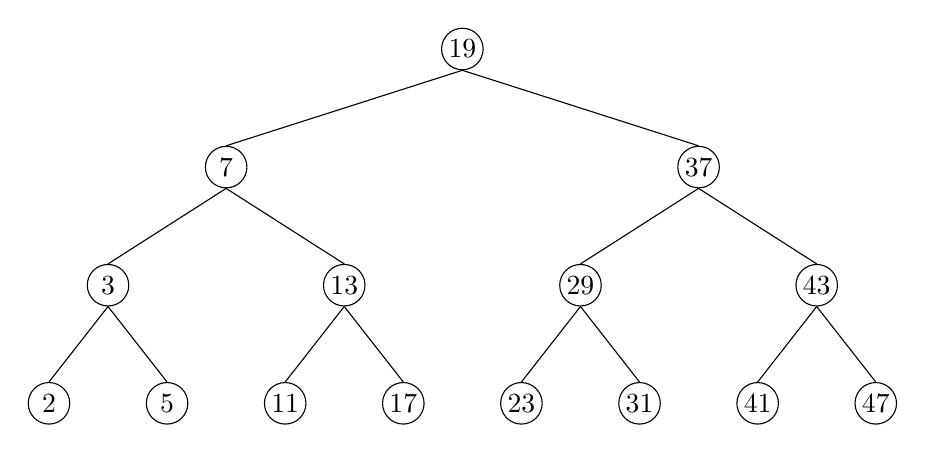
\begin{tikzpicture}[
  level distance=1.5cm,
  level 1/.style={sibling distance=6cm},
  level 2/.style={sibling distance=3cm},
  level 3/.style={sibling distance=1.5cm},
  every node/.style={circle, draw, minimum size=1.5em, inner sep=1pt}
]

\node {19}
  child {node {7}
    child {node {3}
      child {node {2}}
      child {node {5}}
    }
    child {node {13}
      child {node {11}}
      child {node {17}}
    }
  }
  child {node {37}
    child {node {29}
      child {node {23}}
      child {node {31}}
    }
    child {node {43}
      child {node {41}}
      child {node {47}}
    }
  };

\end{tikzpicture}

\break

\section*{Aufgabe 6.4}
\subsection*{a)}
Fügen Sie die Schlüssel
\begin{center}
    21, 15, 5, 33, 28, 30\\
\end{center}
in dieser Reihenfolge in einen anfangs leeren AVL-Baum ein. Stellen Sie den Baum inklusive der Balancegrade aller Knoten nach jeder Einfüge-Operation dar. Sofern nach einer Einfügung (mindestens) eine Rotation notwendig ist, stellen Sie den Baum zusätzlich vor jeder Rotation dar. Geben Sie in diesem Zusammenhang außerdem an, welcher Rotationsfall (Zick-Zick, Zick-Zack, Zack-Zick oder Zack-Zack) vorliegt und welche Rotation(en) ausgeführt wird bzw. werden.\\

\textbf{1.} $21$\\

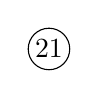
\begin{tikzpicture}[
  level distance=1.5cm,
  level 1/.style={sibling distance=6cm},
  level 2/.style={sibling distance=3cm},
  level 3/.style={sibling distance=1.5cm},
  every node/.style={circle, draw, minimum size=1.5em, inner sep=1pt}
]

\node {21};

\end{tikzpicture}

\textbf{2.} $15$\\

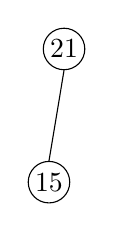
\begin{tikzpicture}[
  level distance=1.5cm,
  level 1/.style={sibling distance=6cm},
  level 2/.style={sibling distance=3cm},
  level 3/.style={sibling distance=1.5cm},
  every node/.style={circle, draw, minimum size=1.5em, inner sep=1pt}
]

\node {21}
    child[anchor=north east] {
        node{15}
    };

\end{tikzpicture}

\textbf{3.} $5$\\

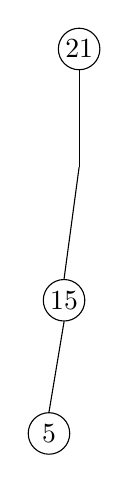
\begin{tikzpicture}[
  level distance=1.5cm,
  level 1/.style={sibling distance=6cm},
  level 2/.style={sibling distance=3cm},
  level 3/.style={sibling distance=1.5cm},
  every node/.style={circle, draw, minimum size=1.5em, inner sep=1pt}
]

\node {21}
    child[anchor=north east] {
        child{node{15}
            child{node{5}
            }
        }
    };

\end{tikzpicture}

\textbf{Zick-Zack (Rechts-Rotation):}\\

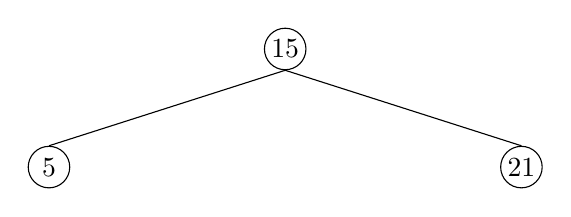
\begin{tikzpicture}[
  level distance=1.5cm,
  level 1/.style={sibling distance=6cm},
  level 2/.style={sibling distance=3cm},
  level 3/.style={sibling distance=1.5cm},
  every node/.style={circle, draw, minimum size=1.5em, inner sep=1pt}
]

\node {15}
      child {node {5}}
      child {node {21}
      };

\end{tikzpicture}

\textbf{4.} $33$\\

\begin{tikzpicture}[
  level distance=1.5cm,
  level 1/.style={sibling distance=6cm},
  level 2/.style={sibling distance=3cm},
  level 3/.style={sibling distance=1.5cm},
  every node/.style={circle, draw, minimum size=1.5em, inner sep=1pt}
]

\node {15}
      child {node {5}}
      child {node {21}
             child[anchor=north west] {node{33}}
      };

\end{tikzpicture}

\textbf{Zick-Zack (Rechts-Rotation):}\\

\begin{tikzpicture}[
  level distance=1.5cm,
  level 1/.style={sibling distance=6cm},
  level 2/.style={sibling distance=3cm},
  level 3/.style={sibling distance=1.5cm},
  every node/.style={circle, draw, minimum size=1.5em, inner sep=1pt}
]

\node {15}
      child {node {5}}
      child {node {33}
             child[anchor=north east] {node{21}}
      };

\end{tikzpicture}

\textbf{5.} $28$\\

\begin{tikzpicture}[
  level distance=1.5cm,
  level 1/.style={sibling distance=6cm},
  level 2/.style={sibling distance=3cm},
  level 3/.style={sibling distance=1.5cm},
  every node/.style={circle, draw, minimum size=1.5em, inner sep=1pt}
]

\node {15}
      child {node {5}}
      child {node {33}
             child[anchor=north east] {node{21}
             child[anchor=north west] {node{28}}}
      };

\end{tikzpicture}

\textbf{Zick-Zick (Rechts-Rotation):}\\

\begin{tikzpicture}[
  level distance=1.5cm,
  level 1/.style={sibling distance=6cm},
  level 2/.style={sibling distance=3cm},
  level 3/.style={sibling distance=1.5cm},
  every node/.style={circle, draw, minimum size=1.5em, inner sep=1pt}
]

\node {15}
      child {node {5}}
      child {node {21}
            child {node{28}
            child[anchor=north west] {node{30}}}
             child {node{33}
             }
      };

\end{tikzpicture}

\textbf{(Links-Rotation)}

\begin{tikzpicture}[
  level distance=1.5cm,
  level 1/.style={sibling distance=6cm},
  level 2/.style={sibling distance=3cm},
  level 3/.style={sibling distance=1.5cm},
  every node/.style={circle, draw, minimum size=1.5em, inner sep=1pt}
]

\node {15}
      child {node {5}}
      child {node {30}
            child {node{21}
            child[anchor=north west] {node{28}}}
             child {node{33}
             }
      };

\end{tikzpicture}

\subsection*{b)}
Betrachten Sie die im Folgenden explizit dargestellte Doppelrotation für einen AVL-Baum (Zick-Zack-Fall). Die Bezeichnungen w, v, u und x geben die Adresse des jeweiligen Knotens im Speicher an. Wir nehmen an, dass jeder Knoten im Baum zwei Zeiger besitzt, links und rechts, die auf das linke bzw. rechte Kind des Knotens zeigen. Geben Sie eine gültige Folge von notwendigen Zeigeraktualisierungen für diese Doppelrotation an. Sie brauchen Ihre Antwort nicht weiter zu begründen.

\begin{verbatim}
    x.rechts = w.rechts
    x.links = w.links
    w.links = v.links
    v.rechts = B1
    v.links = B2
\end{verbatim}



\end{document}